\documentclass[12pt]{article}
\usepackage{graphicx}
\usepackage{setspace}
\usepackage{geometry}
\usepackage{float}
\usepackage{changepage}
\usepackage{indentfirst}

% Support for references.
\usepackage[backend=biber,style=ieee]{biblatex}
\addbibresource{refs.bib}

% Convert references, table of contents and list of figures to links.
\usepackage[colorlinks=false,pdfborder={0 0 0}]{hyperref}

% Make URLs blue and the same font as the rest of the document.
\hypersetup{colorlinks=true,linkcolor=black,urlcolor=blue,citecolor=black}
\urlstyle{rm}

% ... except for References section.
\AtBeginBibliography{%
  \hypersetup{urlcolor=black}
  \urlstyle{tt}
}

% Remove vertical space between TOC items
\usepackage{tocloft}
\setlength{\cftbeforesecskip}{12.5pt}   % sections
\setlength{\cftbeforesubsecskip}{1.5pt} % subsections
\setlength{\cftbeforesubsubsecskip}{1pt} % sub-subsections

% Make captions look better.
\usepackage[labelfont={bf, it},textfont=it]{caption}

% Support for glossaries.
\usepackage[acronym]{glossaries}
\newacronym{nfc}{NFC}{Near-Field Communication}
\newacronym{rfid}{RFID}{Radio Frequency Identification}
\newacronym{ui}{UI}{User Interface}
\newacronym{ux}{UX}{User Experience}
\newacronym{api}{API}{Application Programming Interface}
\newacronym{ssh}{SSH}{Secure Shell}
\newacronym{sftp}{SFTP}{File Transfer Protocol over Secure Shell}
\newacronym{spa}{SPA}{Single Page Application}
\newacronym{url}{URL}{Uniform Resource Locator}
\newacronym{lcd}{LCD}{Liquid Crystal Display}
\newacronym{vps}{VPS}{Virtual Private Server}
\newacronym{dto}{DTO}{Data Transfer Object}
\newacronym{orm}{ORM}{Object-Relational Mapper}


% Don't use long forms.
\AtBeginDocument{\glsunsetall}

% Custom glossary styles.
\renewcommand*{\glossarysection}[2][]{\par\noindent\vspace{-\baselineskip}}
\newglossarystyle{gridtable}{
  \renewcommand*{\glsgroupheading}[1]{}
  \renewenvironment{theglossary}{
    \par\noindent\raggedright
    \begin{tabular}{|p{0.15\textwidth}|p{0.5\textwidth}|}
    \hline
    \textbf{Term} & \textbf{Definition} \\ \hline
  }{
    \end{tabular}
  }
  \renewcommand*{\glossentry}[2]{
    \unskip\glstarget{##1}{\glossentryname{##1}} & \glossentrydesc{##1}\unskip \\ \hline
  }

  % Ignore subentries
  \renewcommand*{\subglossentry}[3]{}
}


% Make glossaries.
\makeglossaries

% Page settings
\geometry{margin=1in}

% Document metadata
\title{CNG 495 Term Project Progress Report}
\date{November 30, 2025}

% 1.5 line spacing entire document
\onehalfspacing 



\begin{document}

% === Title page ===
\begin{titlepage}
    \begin{center}
        
\includegraphics[width=\textwidth]{img/metu.png}
    \end{center}
    \begin{center}
        \Huge\bfseries CNG 495 Cloud Computing \\ Fall 2025-2026 Semester \\ Term Project Progress Report
    \end{center}

    \vfill
    \vfill
    
    {
        \large
        \begin{tabular}{@{} l l @{}}
            \textbf{Project Name}: & RFID-based Attendance System \\
            \textbf{Team Members}: & Can Özkan  - 2638112 \\
                                   & Umut Şen - 2585420 \\
        \end{tabular}
    }

    \vfill
\end{titlepage}


\renewcommand{\contentsname}{Table of Contents} % Rename "Contents" to "Table of Contents"
\tableofcontents
\vspace{1.5em}
\listoffigures
\vspace{1.5em}
\listoftables
\newpage



\section{Project Description}
Our project aims to simplify and automate the process of taking attendance using student ID cards by reducing human interaction. Our system consists of an \gls{nfc} reader hardware, a cloud server that processes attendance \& timetable data, and two distinct web-based \glspl{ui}, for instructors and administrators.\par

Instructors can login to the system using their METU credentials. The interface lets them see how many registered students have arrived, how many are absent and the total number of students registered to the classroom, in a simple interface. In case of a hardware failure, or simply a student forgetting to scan their ID, the instructor can mark a student present too, during or after the lecture hours. Similarly, the instructor can mark a student absent even if the ID card was scanned.\par

The administration panel is strictly to be used by administrators (such as the registrar's office) to monitor the \gls{rfid} readers, assign them to classrooms and view system logs.\par



\section{Implementation}
Times of each lecture, and in which classroom they are taking place are automatically pulled from the university’s timetable system. When a student arrives at the classroom, they are required to scan their ID cards to the \gls{rfid} reader. Scanned \gls{rfid} data is then sent to the cloud server to register attendance. \gls{rfid} reader has both visual and audio elements to give feedback. Students must scan their ID until the lecture time is over for their attendance to be valid. This process can be seen on \autoref{fig:activity}.\par

Our project will use ASP.NET as the backend framework, Supabase as the database and React on GitHub Pages for the frontend design of the cloud part. For the hardware part, we utilize an RC522 \gls{rfid} module to scan ID cards, ESP32-DevKit-V1 module to transmit ID to the cloud, an \gls{lcd} screen and a buzzer to provide feedback.\par

Interaction between services of our project can be seen on \autoref{fig:context}.

\begin{figure}[H]
    \centering
    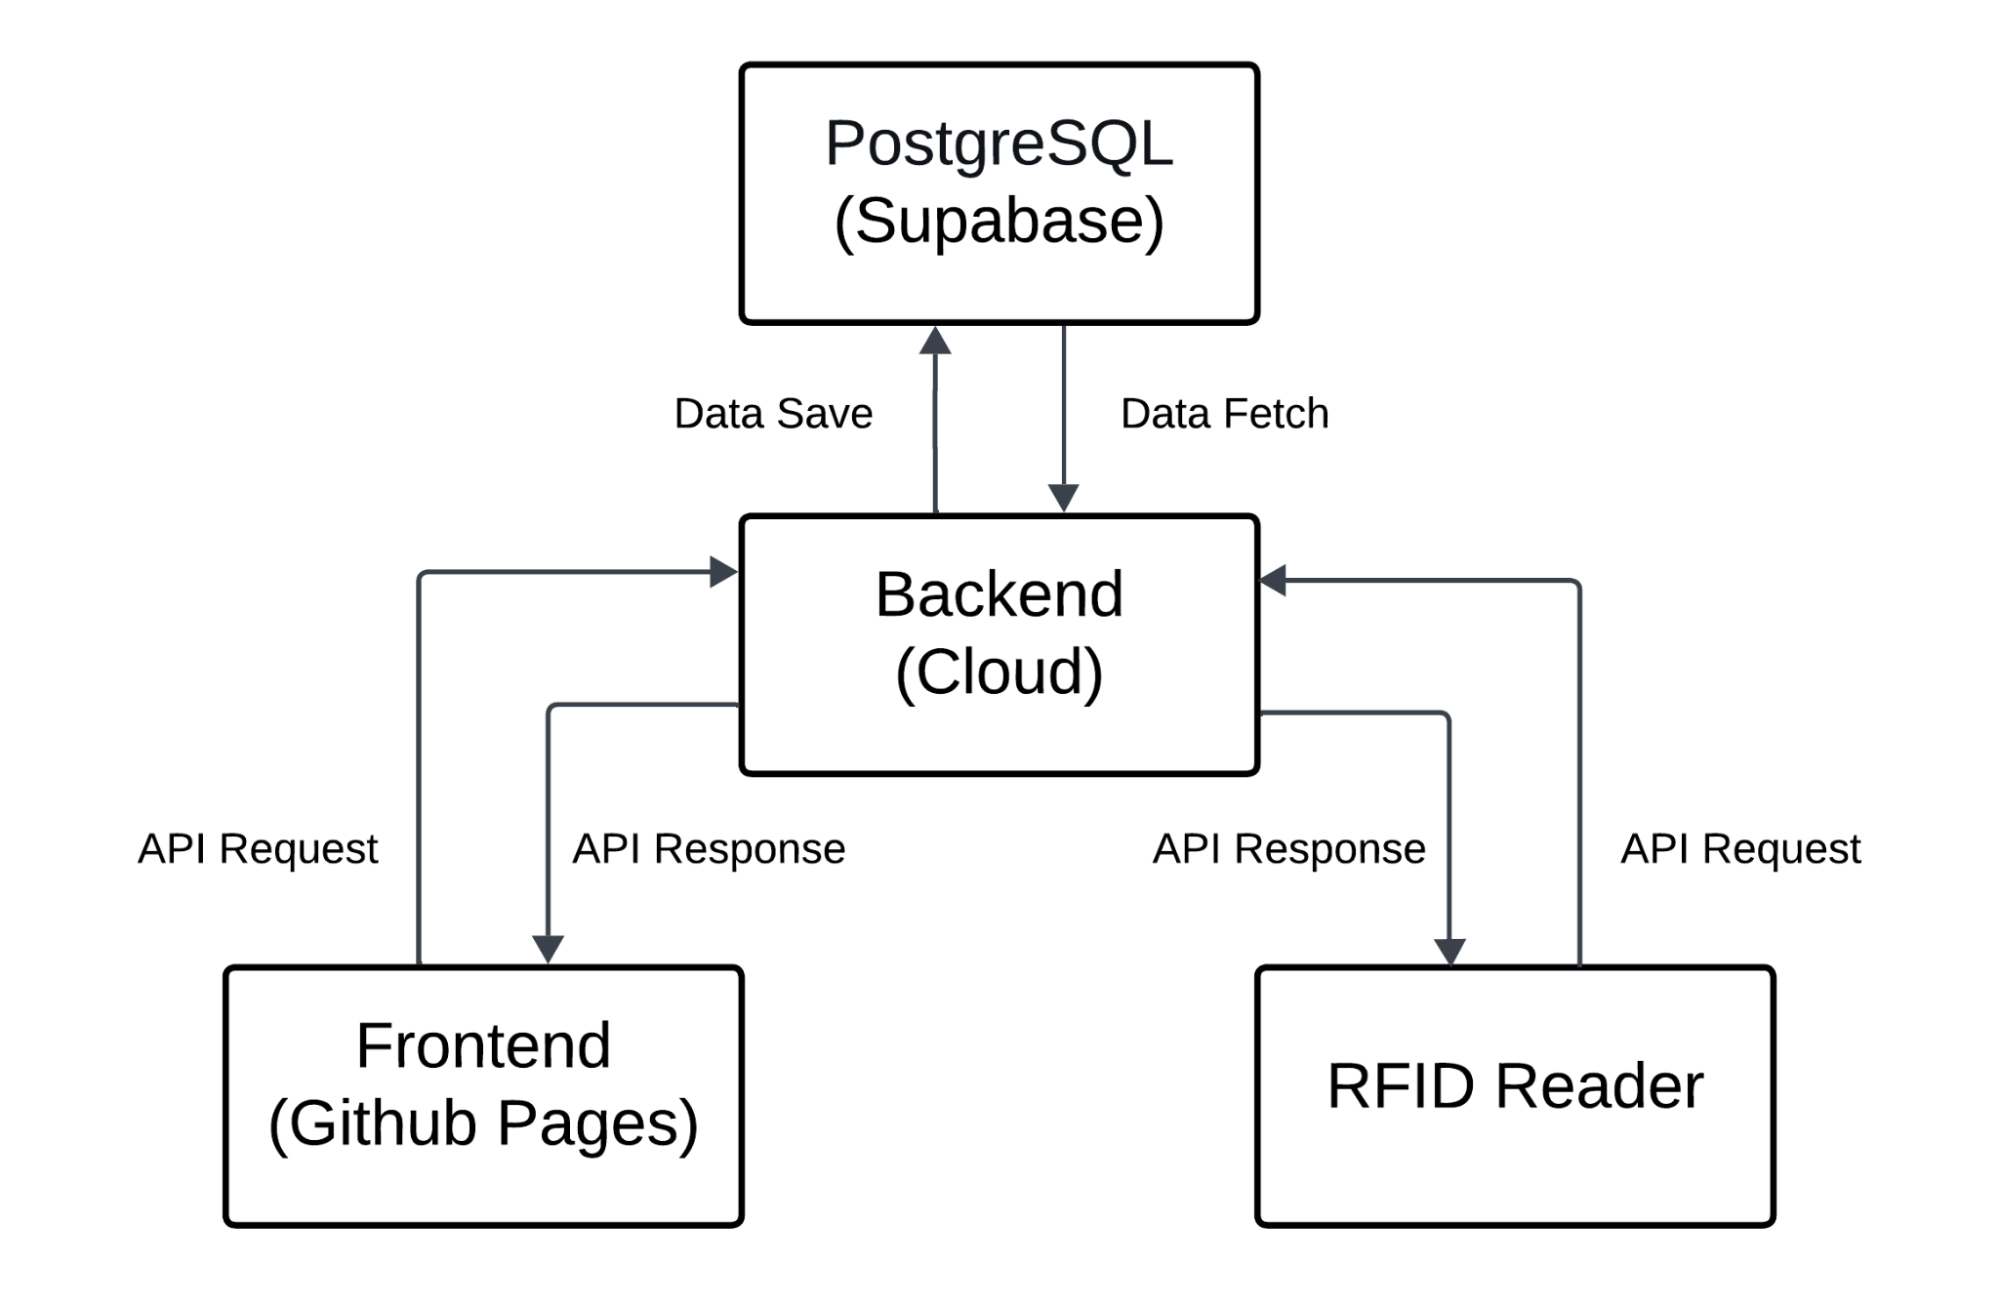
\includegraphics[width=\linewidth]{img/diagram/context.png}
    \caption{System interactions.}
    \label{fig:context}
\end{figure}



\section{Delivery Models}

\subsection{Platform-as-a-Service (PaaS)}
Frontend for our project will be hosted on GitHub Pages, and the database will be served on Supabase Hosted.\supercite{github-pages,supabase-docs}

\subsection{Infrastructure-as-a-Service (IaaS)}
Our backend will run on a virtual private server with a Linux-based operating system.\supercite{vps-com-tr}



\newpage
\section{Data Types}
Our project utilizes various data types to exchange and store information. Data types used in our project are detailed below, categorized by the group they’re used in.

\begin{itemize}
    \item \textbf{Text:} Student full name, Instructor full name, Classroom name, Hardware IP address
    \item \textbf{Number:} Student ID number
    \item \textbf{Timestamp:} Lecture start/end timestamps
    \item \textbf{Binary:} ID card data, hardware keys
\end{itemize}



\section{Computation}
Following computations are made throughout the lifetime of our system:

\begin{itemize}
    \item \textbf{Attendance Recording:} Student attendance is recorded and present \& absent student counts are calculated.
    \item \textbf{User Authentication:} Credentials of parties accessing our system are verified through the METU system.
    \item \textbf{Hardware Authentication:} To prevent unauthorized attendance recording to our system, we check the authenticity of requests coming from all \gls{rfid} readers.
\end{itemize}



\section{Expected Contribution}
\begin{itemize}
    \item \textbf{Hardware Design \& Implementation:} Can Özkan
    \item \textbf{Database Design:} Both students
    \item \textbf{Backend Development:} Both students
    \item \textbf{Frontend Development:} Umut Şen
\end{itemize}



\newpage
\section{Diagrams}
This section contains various diagrams that visualize how our system works.

\subsection{Activity Diagram}

\begin{figure}[H]
    \centering
    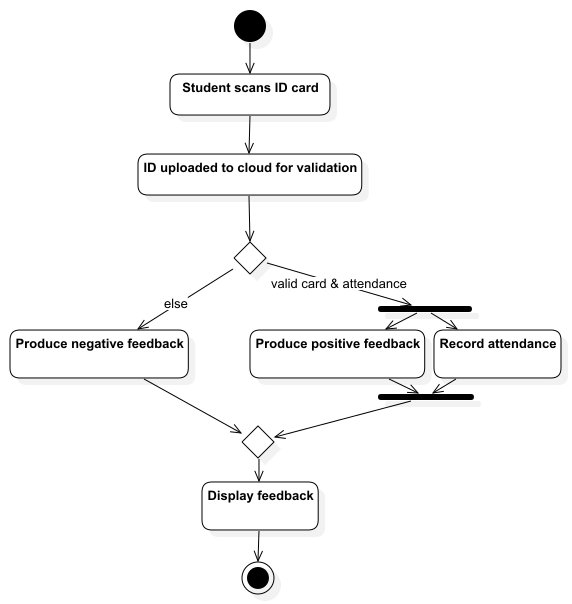
\includegraphics[width=\linewidth]{img/diagram/activity.png}
    \caption{Student ID \& attendance verification process.}
    \label{fig:activity}
\end{figure}


\newpage
\subsection{Use Case Diagram}

\begin{figure}[H]
    \centering
    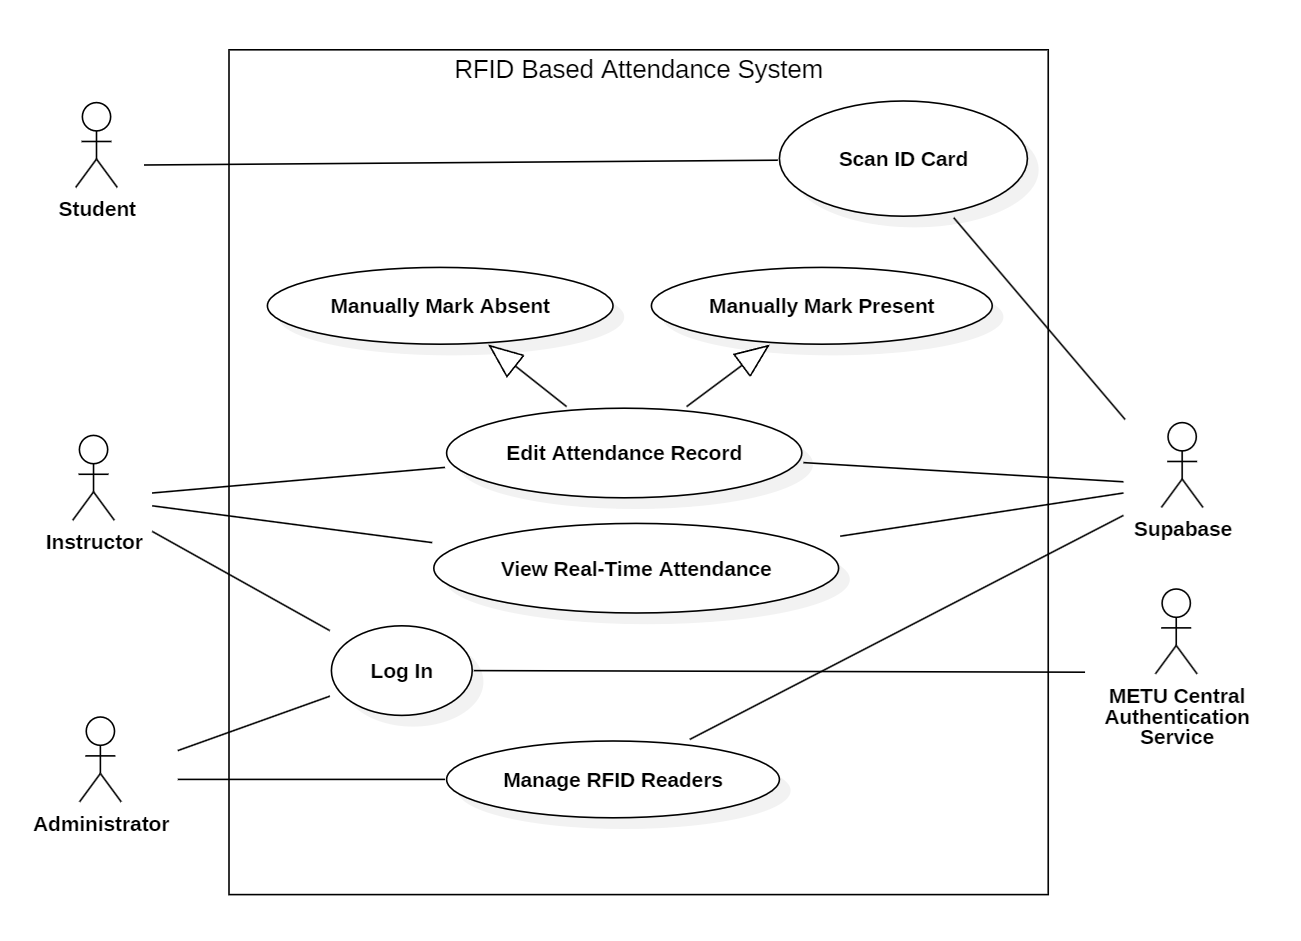
\includegraphics[width=\linewidth]{img/diagram/usecase.png}
    \caption{Use case diagram.}
    \label{fig:usecase}
\end{figure}


\newpage
\subsection{Data Flow Diagram}

\begin{figure}[H]
    \centering
    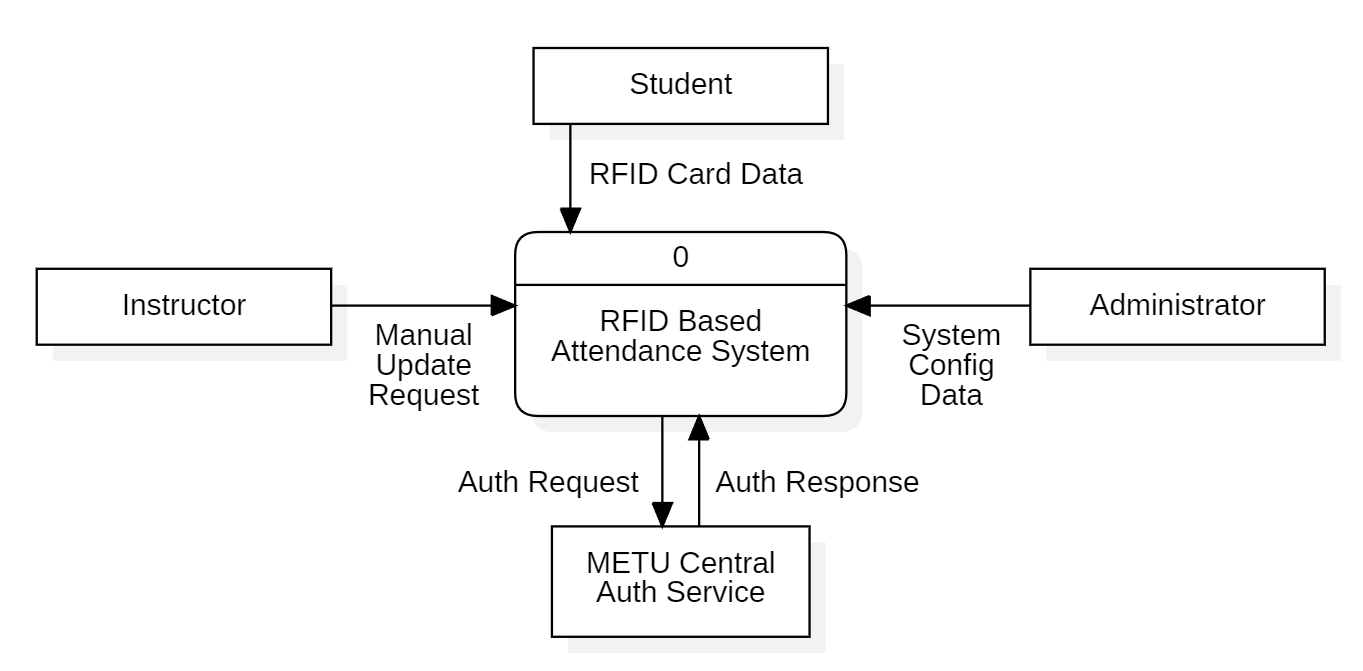
\includegraphics[width=0.75\linewidth]{img/diagram/dfd0.png}
    \caption{Level 0 data flow diagram.}
    \label{fig:dfd0}
\end{figure}

\begin{figure}[H]
    \centering
    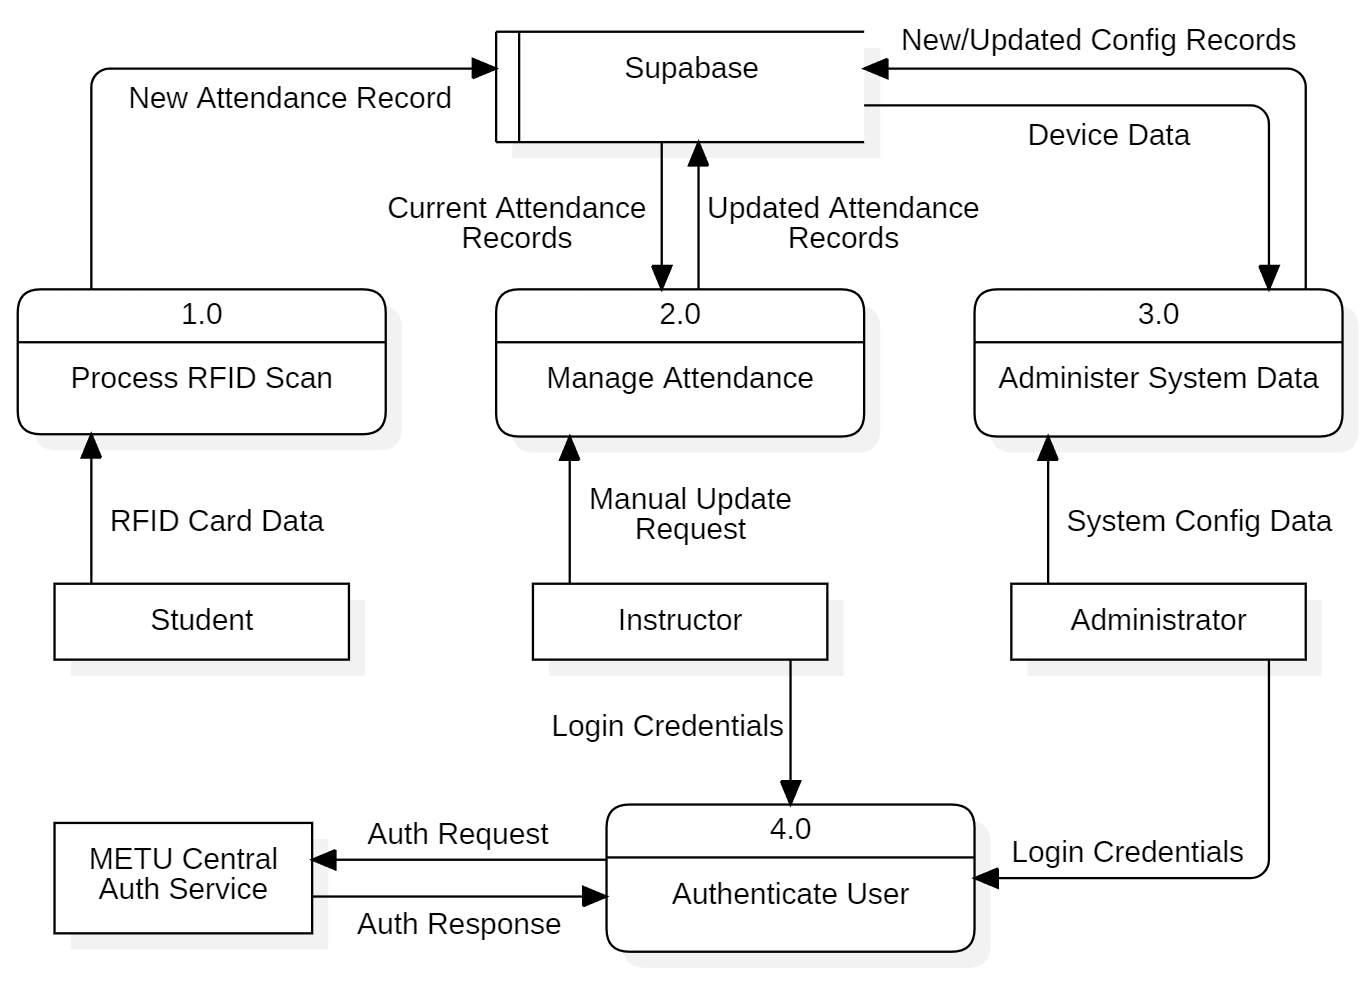
\includegraphics[width=0.75\linewidth]{img/diagram/dfd1.png}
    \caption{Level 1 data flow diagram.}
    \label{fig:dfd1}
\end{figure}



\newpage
\section{Milestones Achieved}
This section is divided into two parts: Milestones achieved by Umut and Milestones achieved by Can. Additionally, each part categorizes milestones and tasks done by term weeks.


\subsection{Milestones Achieved by Umut}


\subsubsection{Week 4 (20 October - 26 October)}
First, I tried some page layouts in a random React project. After selecting some good components, I created a new React Router project and migrated them over. While doing that, I also tried using TanStack Query and decided to stick with it, and created \gls{api} functions for the components I made.
\begin{figure}[H]
    \centering
    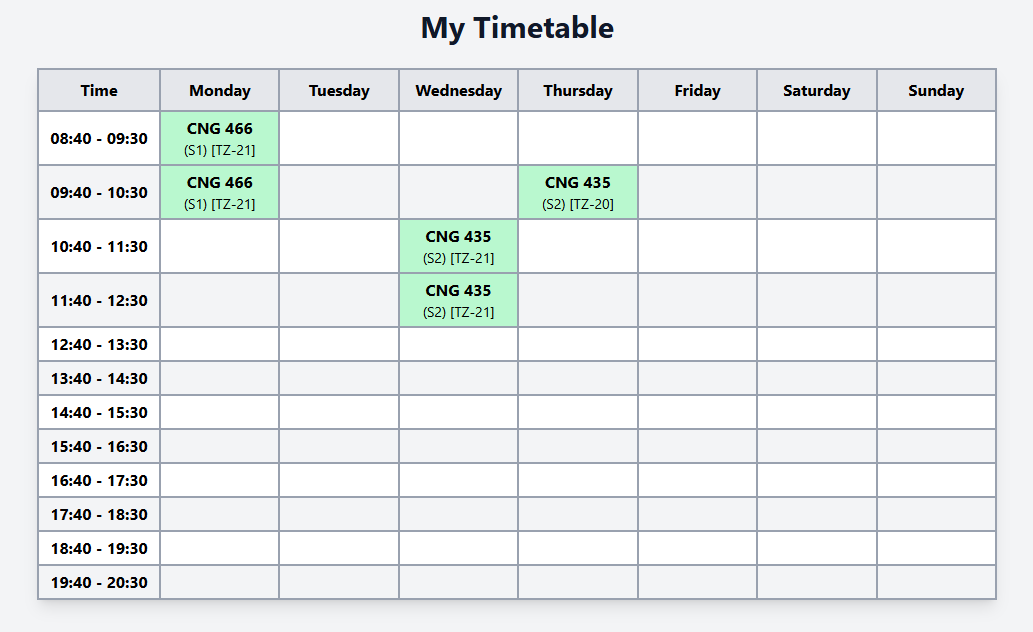
\includegraphics[width=\textwidth]{img/sshot/timetables_first.png}
    \caption{First iteration of timetables.}
    \label{fig:ttablef}
\end{figure}

\begin{figure}[H]
    \centering
    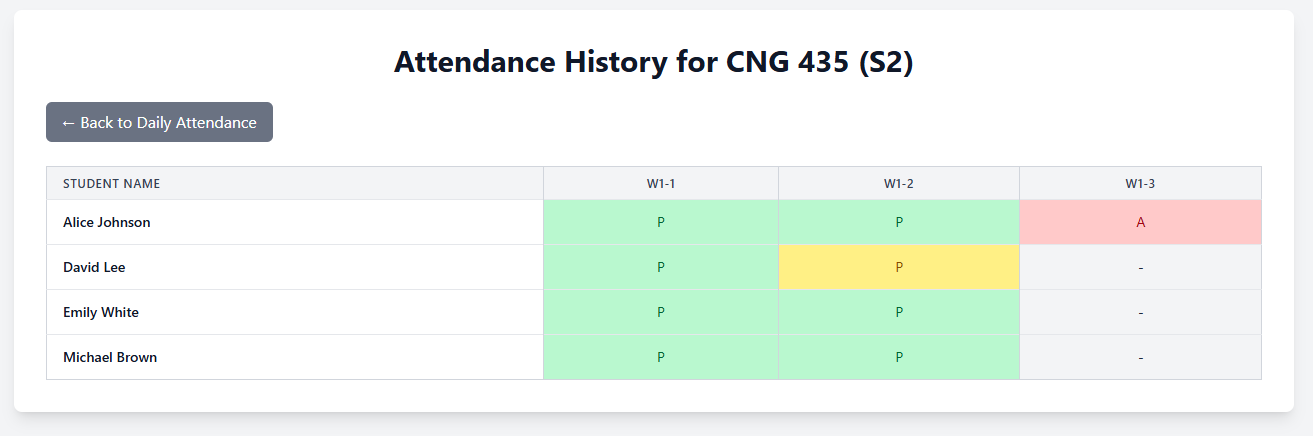
\includegraphics[width=\textwidth]{img/sshot/fhistory_first.png}
    \caption{First iteration of full history.}
    \label{fig:fhistoryf}
\end{figure}

\autoref{fig:ttablef} and~\autoref{fig:fhistoryf} show the state of the components I made during the first week. They are fundamental components with fixed test parameters. They were made to see what the \glspl{ui} could look like and how the user flow could feel.

\subsubsection{Week 5 (27 October - 2 November)}
This week, I worked on the live attendance system that used WebSockets. I implemented it using the socket-io library, but I later changed it. Also, I created the general design and the \gls{ux} of the live attendance page. Lastly, to test it, I created a mock backend in Python with some fake data.
\begin{figure}[H]
    \centering
    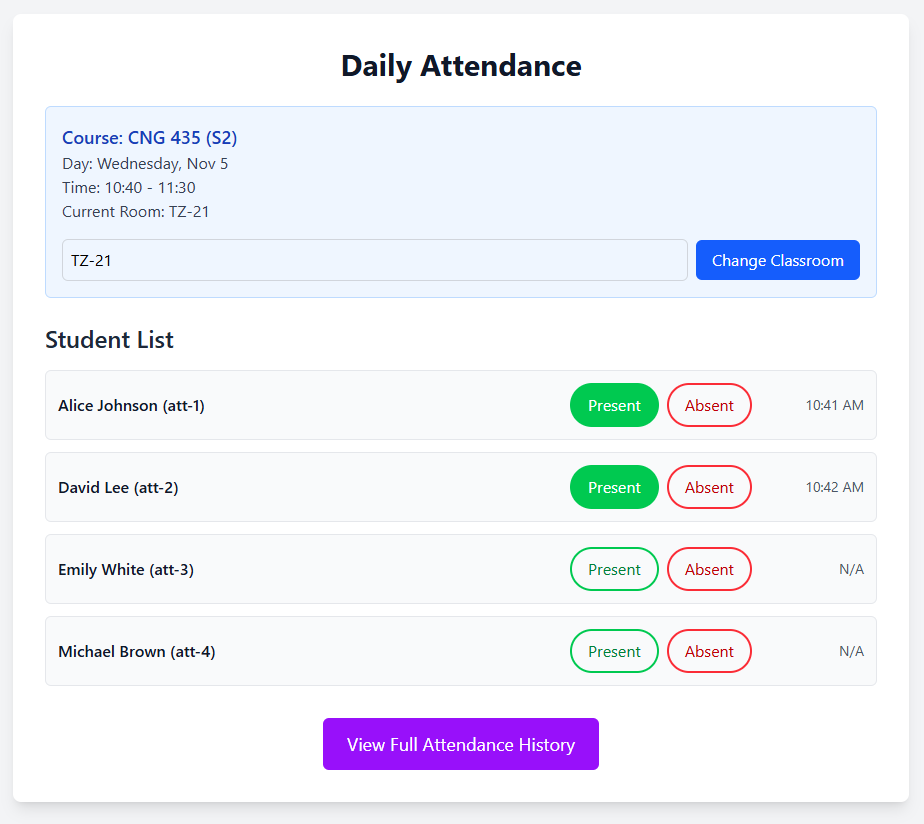
\includegraphics[width=\textwidth]{img/sshot/liveas_first.png}
    \caption{First iteration of live attendance system.}
    \label{fig:liveasf}
\end{figure}

You can see the initial design of the live attendance system in~\autoref{fig:liveasf}. We really liked the general layout of this one, so we kept it for the later versions.

\subsubsection{Week 6 (3 November - 9 November)}
We had exams starting in about a week, so I didn't have much time to spend on this project. I mainly cleaned up and refactored components to make the project more modular.
There is not much to show here, but an example is the "api.ts" file inside the \verb|/frontend/src/lib| directory. I created it while refactoring to clean up the components and to separate the data from the \gls{ui}.

\subsubsection{Week 7 (10 November - 16 November)}
Didn't really do anything this week since we had many exams and other projects all colliding.

\subsubsection{Week 8 (17 November - 23 November)}
Again, we had exams at the start of the week, so I didn't do that much, but I decided to switch to another framework. I decided to use the TanStack Router instead of the React Router since we were already using TanStack Query for our data. It was the better option for the project. In short, I migrated all my components and pages to a new project built with TanStack Router. 
The reason I chose to use the TanStack Router is that the type safety of the TanStack Query is already excellent on its own, and when combined with the TanStack Router, the project becomes type-safe all the way through, including routes and imports. At the beginning of the project, I underestimated its complexity, so I expected React Router would be enough. But it started to get cluttered, and switching to TanStack Router solved that problem.

\subsubsection{Week 9 (24 November - 30 November)}
This week, I created a basic style for the app and updated all my components and pages to use it. Also, I realized that to better fit with the backend, I should have used the native WebSocket \gls{api}, so I switched to it. In anticipation of the report, I deployed the frontend, which is about 50\% complete, to GitHub Pages using a script I wrote. I had to write a custom script for it since our repository was private, and you cannot use GitHub Pages on a private repository unless you are a paid member. So I created a public repository and wrote a script that builds only the frontend and serves it via GitHub Pages.
\begin{figure}[H]
    \centering
    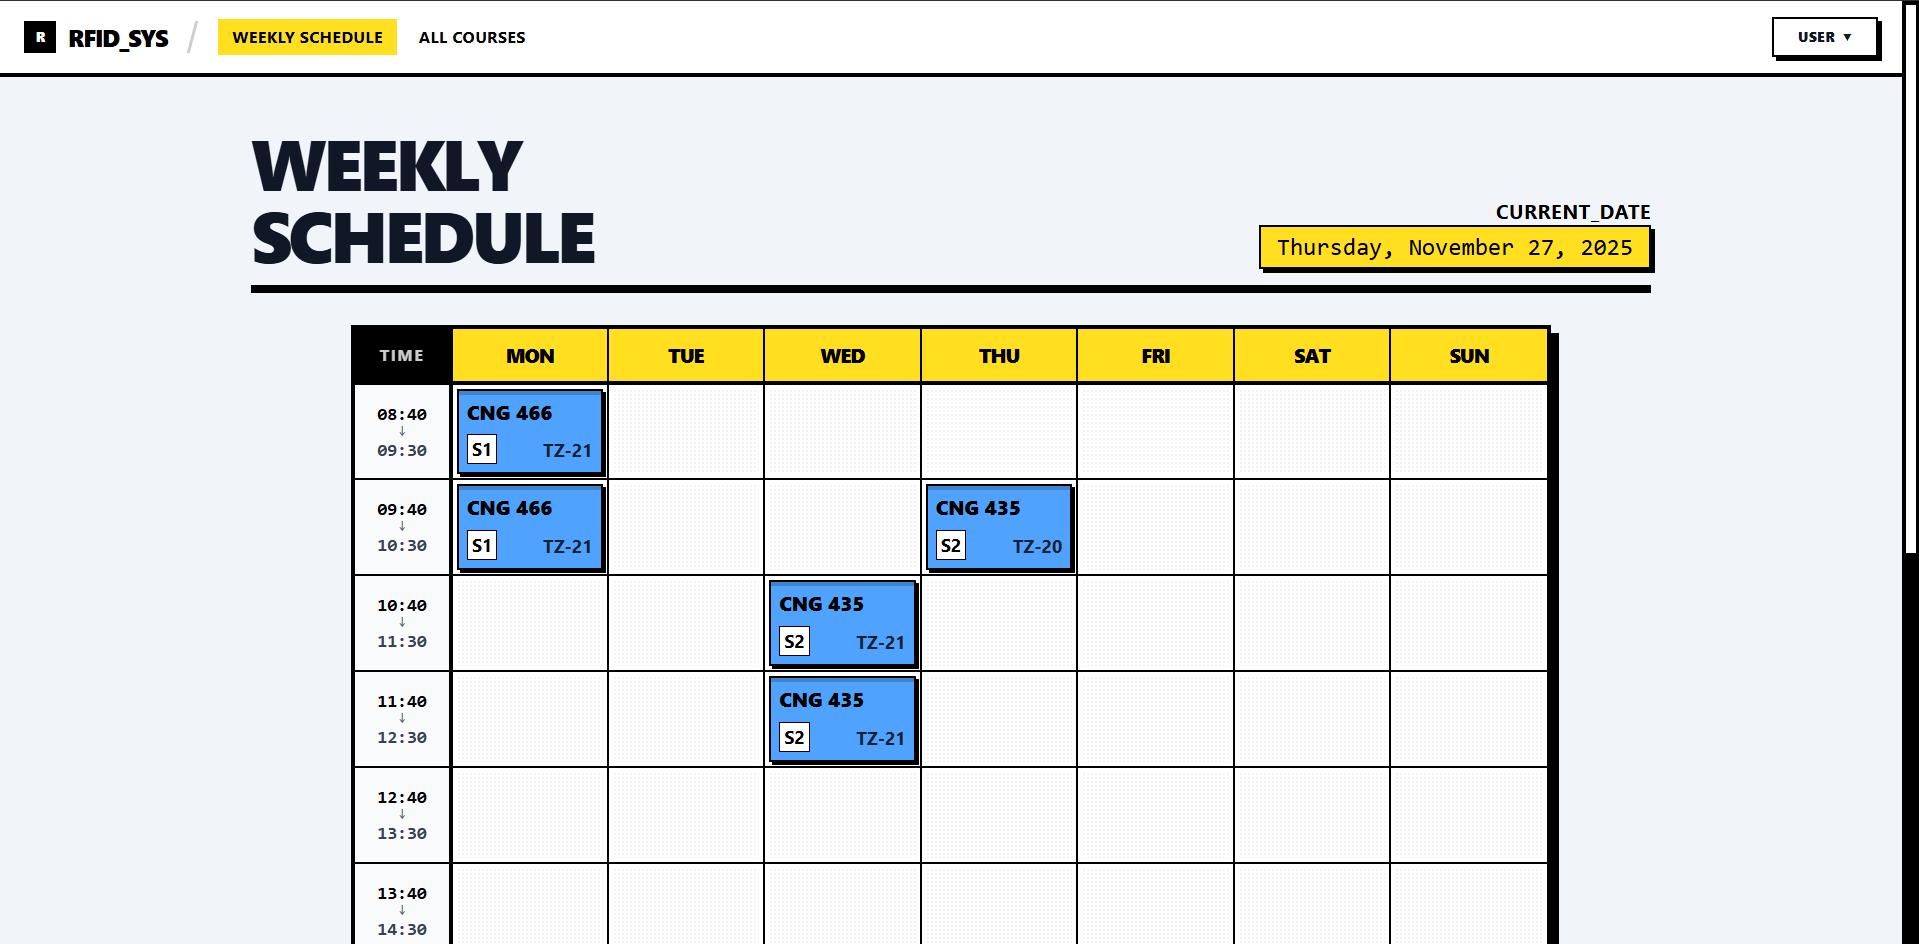
\includegraphics[width=\textwidth]{img/sshot/timetables_second.png}
    \caption{The weekly schedule screen with the new and improved timetable.}
    \label{fig:ttables}
\end{figure}

\begin{figure}[H]
    \centering
    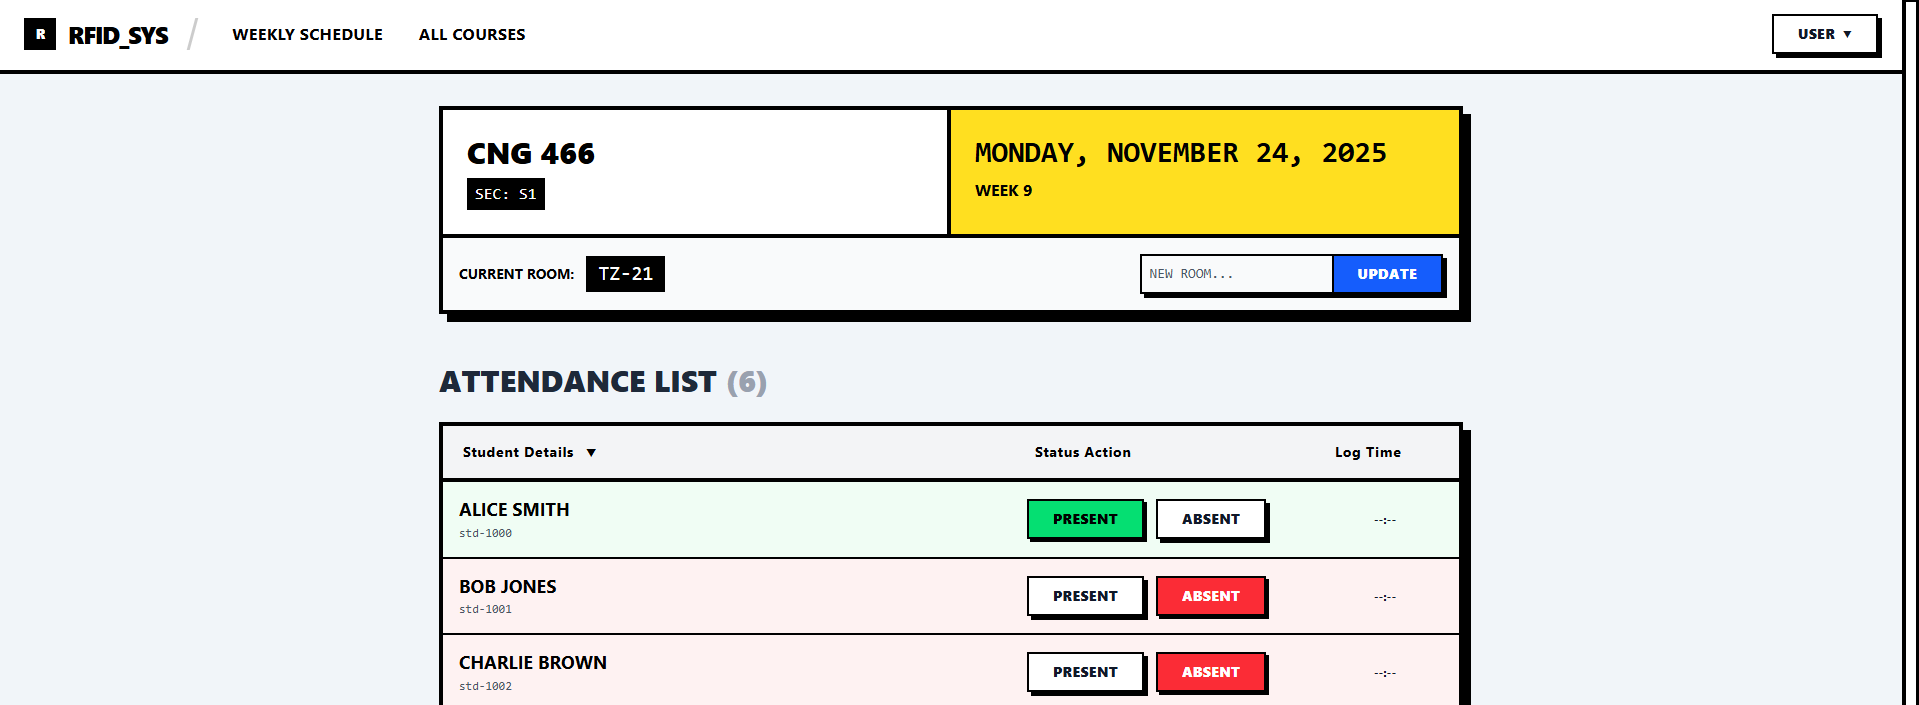
\includegraphics[width=\textwidth]{img/sshot/liveas_second.png}
    \caption{The live attendance tracking system with the new boxy style.}
    \label{fig:liveass}
\end{figure}

\autoref{fig:ttables} and~\autoref{fig:liveass} show that this redesign not only uses a consistent visual identity but also significantly improves the look compared to the initial prototypes.\par

\vspace{1.5em}
\textbf{Automated CI/CD with GitHub Actions (PaaS)}: I used GitHub Actions to create a pipeline that automatically builds the frontend from our private repository and deploys it to a separate public repository. That way, I don't have to manually build the project on my laptop and upload it to the public repository every time. To do that, I configured a workflow file that triggers on every push to the main branch that affects the frontend file. Here is a step-by-step tutorial to achieve a pipeline like this.

\begin{enumerate}
    \item Generate \gls{ssh} keys for GitHub to use while pushing from the private repository to the public one.
    \item Configure the repositories to use these keys on the public repository. We set up the public \gls{ssh} key as a deploy key and grant it write access. Then, in the private repository, we added the private key as an action secret, visible only to GitHub Actions.
    \item Create the .yml file that determines the workflow. We started by using one of the example workflows GitHub provides for static website deployment. We had to decide when and where to trigger the action and what it would do. For our setup, the action only triggers when the "frontend" folder changes. When a change is detected, it will run the standard \verb|npm run build| command to build the static website. After that, it will push the newly built website to the public repository, at which point another workflow on that repository takes over and automatically serves the page using GitHub Pages.
\end{enumerate}

\vspace{1.5em}
\textbf{Static Hosting with GitHub Pages (SaaS)}: We use GitHub Pages to host the frontend. Since React is a \gls{spa} that handles routing on the client side, standard static hosting breaks when using a sub-page, especially on GitHub Pages, since we have little control over the actual deployment. To solve that problem, I am using hash routing, which adds a \verb|#| before the sub-pages on the \gls{url}, which the browser understands as "Don't send anything after \verb|#| to the server". This allows the website to run on GitHub Pages without any problems while functioning like a multi-page app. The live web page \gls{url} is provided in~\autoref{apx:links}.


\subsection{Milestones Achieved by Can}

\subsubsection{Week 4 (20 October - 26 October)}
Started drafting hardware design and started creating our first device by assembling the ESP32-DevKit-V1 module with an RC522 \gls{rfid} reader to scan the cards and a 20x4 \gls{lcd} module to give visual feedback. After assembling the parts, I wrote code to test whether the \gls{lcd} screen and \gls{rfid} reader were operational, and it was successful.

\subsubsection{Week 5 (27 October - 2 November)}
Changed the hardware assembly to include a speaker for sound feedback. This also defines the last revision on the module hardware.
\begin{figure}[H]
    \centering
    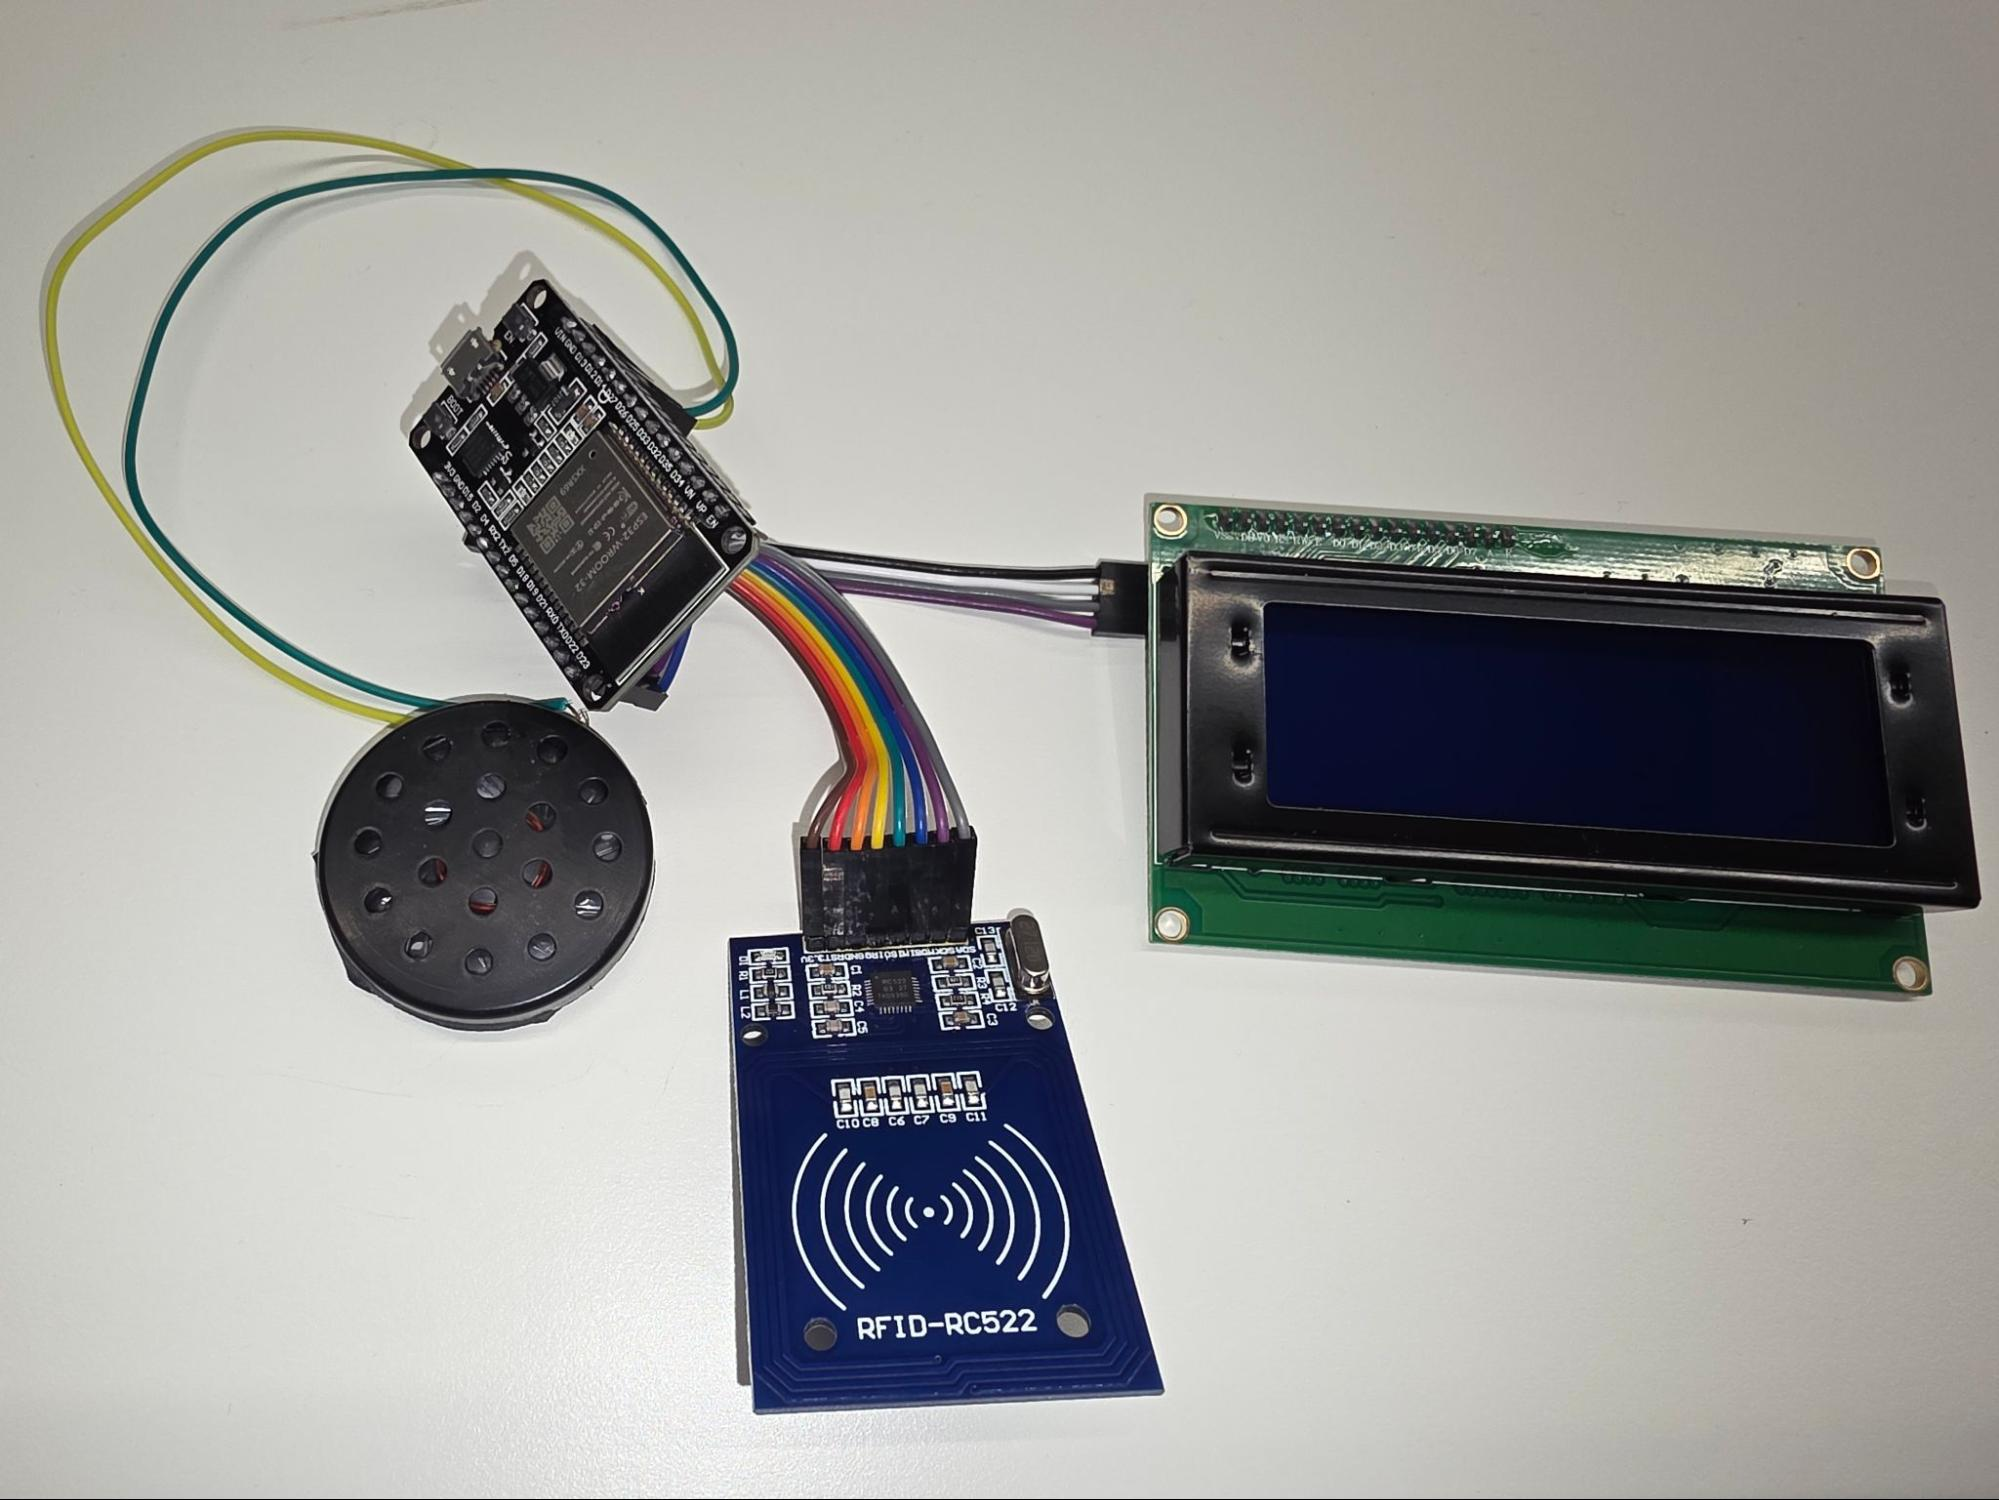
\includegraphics[width=\textwidth]{img/sshot/hardware.jpg}
    \caption{Final assembly of the hardware.}
    \label{fig:hwfinal}
\end{figure}

After assembling the hardware as shown in~\autoref{fig:hwfinal}, I then included the necessary code to make the speaker functional. Once I confirmed that all parts were operational, I restructured the project by splitting features into separate files and modules, then finished the code for the audio player, \gls{lcd} controller, and WebSocket handler, including Wi-Fi connection management.

\subsubsection{Week 6 (3 November - 9 November)}
Determined the database schema \& structure with Umut and, as we follow a code-first approach, represented our tables as classes (models) in C\# so that our \gls{orm} library can automatically generate the database for us. Implemented a short WebSocket testing code at the backend to check if ESP32 can communicate with the backend server, and it was successful.\par
The \gls{vps} we have runs Debian Linux 12. We connect to the machine using \gls{ssh}. To run the test application on it, the following steps were taken:
\begin{enumerate}
    \item Installed ASP.NET Core runtime on it by executing\\\verb|sudo apt install aspnetcore-runtime-10.0|.
    \item Copied deployment files onto the machine using \gls{sftp}.
    \item Executed the application using \verb|dotnet CloudAPI.dll|, where \verb|CloudAPI.dll| is the entry point of our application. This was done in a virtual terminal using GNU Screen\supercite{gnu-screen} to run the application in the background using the following one-liner: \\\verb|screen -S CloudAPI -dm dotnet CloudAPI.dll|.
\end{enumerate}

\subsubsection{Week 7 (10 November - 16 November)}
Parts for the second module arrived. I assembled it and flashed the code to see if the components work correctly. Other than that, no work was done as it was a busy week with midterms, quizzes, and deadlines.

\subsubsection{Week 8 (17 November - 23 November)}
No work done as it was a busy week with midterms, quizzes, and deadlines.

\subsubsection{Week 9 (24 November - 30 November)}
Created many helpers and utilities to process, work, and represent our models \& attributes. Resolved numerous ambiguities in the design of database models that were left unsolved in Week 6. Created the database context, which manages all the operations related to the database. Created migrations, which is basically the “Version Control” of the database structure, so that it is easier to make future changes without breaking existing data. Integrated Supabase connection into the backend server and applied all pending migrations, essentially applying the schema to the database. Created \glspl{dto} for use in \gls{api} responses, and integrated them into models so that it is possible to create \glspl{dto} with a single method call on database models.\par
To create a PostgreSQL database on Supabase, we first had to create a new Supabase account and then create a new project on it. Then, to connect Supabase to our backend, we enabled Shared Pooler\supercite{supabase-connect} so our backend could connect to it over IPv4, since Supabase uses IPv6 for direct connections by default, but our backend does not support IPv6.
And finally, we acquired the connection string from the Supabase dashboard and provided it to our backend to finalize the integration.



\newpage
\section{Milestones Remaining}
Below are the remaining milestones we need to complete.


\subsection{Finish the other half of the frontend pages (Week 10)}
Umut needs to make the general courses screen, the long attendance lists screen, and any other screens we might decide to add while finishing up the project.


\subsection{Create the protocol between backend and devices (Week 10)}
Our hardware and the server need a common language to communicate. Can will design a lightweight binary-based protocol that handles card information to the server and the attendance registration results back to the device.


\subsection{Create \glspl{api} for the frontend (Week 11)}
Can and Umut will create the \gls{api} endpoints needed for \glspl{ui}, and Umut will connect them to the frontend.


\subsection{Create the Admin \gls{ui} (Week 11)}
Finally, Umut will work on and finish the admin \gls{ui}. We are leaving this as the final task to make sure the data structures and features are fully stabilized. This should prevent the need to refactor the admin tools at the last minute for every little change.



\section{Deliverables}
On successful completion of our project, the following deliverables will be produced:
\begin{itemize}
    \item \textbf{Source Code}: The complete source code for the project.
    \item \textbf{\gls{rfid}-Reader Device}: The hardware responsible for scanning the ID cards, sending them to the backend, and displaying back the result of attendance.
    \item \textbf{Deployed Application}: The web page on GitHub Pages \& backend server on a virtual private server.
    \item \textbf{Admin Control Panel}: The control panel to manage devices \& timetable.
    \item \textbf{Final Report}: A document detailing our project.
\end{itemize}



\newpage
\section{Abbreviations}
\begin{table}[H]
    \centering
    \printglossary[type=\acronymtype,style=gridtable,title=Abbreviations]
    \captionof{table}{Table of abbreviations.}
    \label{table:glossary}
\end{table}



\newpage
\printbibliography[title={References}]



\newpage
\appendix
\section{Links}\label{apx:links}
\begin{itemize}
    \item Our source code for the frontend pages, the backend server, and the device is available on GitHub at \url{https://github.com/cnzkn/RFIDAttendanceSystem}. As the repository is private, please get in touch with us to request access.\par
    \item The public repository, hosting the compiled resources for the frontend page, is hosted at \url{https://github.com/UmutSen2662/RFIDAttendanceSystemPages}.\par
    \item The page is hosted live by GitHub Pages at \\\url{https://umutsen2662.github.io/RFIDAttendanceSystemPages/}.
\end{itemize}

\end{document}
